\clearpage\section{Experiments}\label{sec:experiments}
%
\begin{table}[b]
    \centering
    \begin{tabular}{c|ccc|cc}\toprule
        \textbf{Method} & Param. (M) & Size (MB) & Step (ms) & high $\nu$ & low $\nu$ \\
        \midrule
        FFNO \citep{tran2021factorized} & $8.9$ & $35$ & $294$ & $0.997${\small$\pm 0.003$} & $1.016${\small$\pm 0.010$}\\
        FNO \citep{li2020fourier} & $14.2$ & $56$ & $31$ & $0.379${\small$\pm 0.006$} & $0.328${\small$\pm 0.004$} \\
        FNOvp  & $14.2$ & $56$ & $32$ & $0.351${\small$\pm 0.003$} & $0.315${\small$\pm 0.006$} \\ 
        \rowcolor{blue!4}
        \ourmethod{+vp} & $10.2$ & $40$ & $19$ & $\textbf{0.257}${\small$\pm 0.007$} & $\textbf{0.240}${\small$\pm 0.004$} \\
    \end{tabular}
    \vspace{1mm}
    \caption{\small Benchmarks on incompressible Navier-Stokes. Direct long-range prediction errors (N-MSE) in $n$-space (signal space) of different models.}
    \label{tab:ns}
\end{table}
%
We validate \ourmethod{} on learning to approximate solution operators of dynamical systems from images. 
\begin{itemize}[leftmargin=5.5mm]
    \item In \cref{subsec:ns}, we apply \ourmethod{} on the standard task of learning solution operators for incompressible Navier-Stokes, comparing against other FDMs. In \cref{subsubsec:ns_ab} we perform a series of ablation experiments on each ingredient of the \ourmethod{} recipe, including weight initialization and architecture. In \cref{subsubsec:ns_sl} we provide scaling laws.
    \item In \cref{subsec:dfp} we deal with fluid-solid interaction dynamics in the form of higher resolution images ($128$). We consider turbulent flows around varying airfoil geometries, benchmarking against current SOTA \citep{thuerey2020deep}.
    \item In \cref{subsec:scal} we show how the computational efficiency of \ourmethod{} allows learning on unwieldy data without downsampling or building low-resolution meshes. We consider learning on high-resolution video ($600$ × $1062$) capturing the turbulent dynamics of smoke \citep{eckert2019scalarflow}.
\end{itemize} 

Configuration and model details are reported in the supplementary material. The code is available at \url{https://github.com/DiffEqML/kairos}. \textit{Weights \& Biases} ({\tt wandb}) \citep{wandb} logs of results are provided. 


\subsection{Incompressible Navier-Stokes}\label{subsec:ns}
%
We show that \ourmethod{} matches or outperforms SOTA FDMs with less computation on the standard incompressible Navier-Stokes benchmark. Losses are reported in $n$-space (signal space) for comparison.

\paragraph{Setup}
We consider two-dimensional Navier-Stokes equations for incompressible fluid in vorticity form as described in \citep{li2020fourier}. Given a dataset of initial conditions, we train all models to approximate the solution operator at time $50$ seconds for high viscosity ($\nu = 1e^{-3}$) and at time $15$ for lower viscosity ($\nu = 1e^{-4}$). As a metric, we report \textit{normalized mean squared error} (N-MSE). Both initial condition as well as solution are provided as images of resolution $64$. 

We include as baseline established FDMs, such as Fourier Neural Operators (FNOs) \citep{li2020fourier} and \textit{Factorized Fourier Neural Operators} (FFNOs) \citep{tran2021factorized}. We indicate with the suffix \textit{vp} models that employ the proposed variance preserving initialization scheme. All models truncate to $m=24$, except FFNOs to $m=32$.

\begin{minipage}[t]{\linewidth}
    \centering
    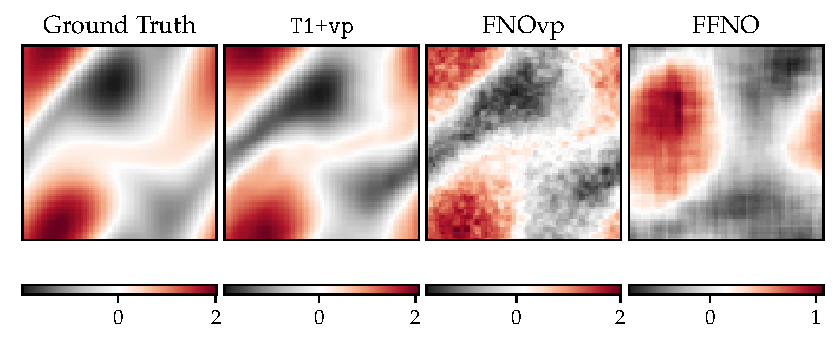
\includegraphics[width=0.49\linewidth]{figures/navier_stokes_physical.pdf}
    \hfill
    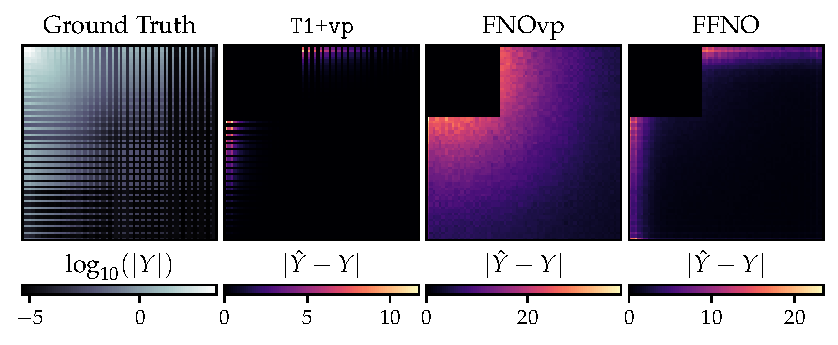
\includegraphics[width=0.49\linewidth]{figures/navier_stokes_dct.pdf}
    \vspace{-3mm}
    \captionof{figure}{\small \textbf{[Left]} Direct predictions at $T=50$s on high viscosity Navier-Stokes. \textbf{[Right]} Ground-truth spectrum and absolute errors in $k$-space (DCT-II). Despite predicting only the first $m=24$ elements, reduced-order \ourmethod{} models produce smaller errors even in other regions of the $k$-space.}
\label{fig:navier}
\end{minipage}

\paragraph{Results}
We perform $20$ training runs for each model and report mean and standard deviation in \cref{tab:ns}. \ourmethod{} reduces solution error w.r.t FNOs by over $20\%$ and FFNOs by over $40\%$. A single forward pass of \ourmethod{} models is on average $2$x faster than FNO and $10$x than FFNOs. We note that FFNOs are designed to share parameters between layers and thus require deeper architectures -- and slower, due to more transforms.  In particular, training time ($500$ epochs) for \ourmethod{} is cut to $20$ minutes down from $40$ of FNOs, matching the model speedup. Finally, we report an improvement in performance for FNOs with parameters initialized following our proposed scheme (FNOvp). \cref{fig:navier} provides sample predictions in $n$-space (left) to contextualize the task, in addition to prediction errors in frequency domain (right). Despite being a reduced order model with $m=24$, \ourmethod{+vp} produces smaller errors on truncated $k$-space elements ($k > m$) compared to FNOvp and FFNO.




\subsubsection{Ablations on weight scheme and architecture}\label{subsubsec:ns_ab}
%
\begin{wraptable}[9]{r}{0.35\linewidth}
    \vspace{-2mm}
    \centering
    \begin{tabular}{c|c|cc}\toprule
        \textbf{Method} & high $\nu$ & low $\nu$\\
        \midrule
        \ourmethod & $0.491$ & $0.449$\\ 
        \ourmethod{vp} & $0.304$ & $0.280$\\ 
        \ourmethod{+} & $0.295$ & $0.260$\\
        \rowcolor{blue!4}
        \ourmethod{+vp} & $\textbf{0.257}$ & $\textbf{0.240}$\\
    \end{tabular}
    \vspace{-1.4mm}
    \caption{\small Ablation on the effect of the proposed weight initialization scheme and \ourmethod{} architecture.}
    \label{tab:ablans}
\end{wraptable}

We repeat the previous experiment and report prediction errors for four variants of \ourmethod{}: same architecture and weight initialization scheme as FNOs (\ourmethod{}), \ourmethod{} with our proposed vp scheme (\ourmethod{vp}), a reduced-order variant with $k$-space model $f_\theta$ defined as a UNet architecture (\ourmethod{+}), and \ourmethod{+} with variance preserving scheme (\ourmethod{+vp}). The results in \cref{tab:ablans} provide empirical evidence in support of the vp scheme and its synergistic effect with the proposed architecture. In particular, combining vp scheme and UNet structure in frequency domain reduces error by half compared to the naive \ourmethod{} approach.
%

\subsubsection{Scaling laws}\label{subsubsec:ns_sl}
%
\begin{wrapfigure}[9]{r}{0.4\linewidth}
    \centering
    \vspace{-10mm}
    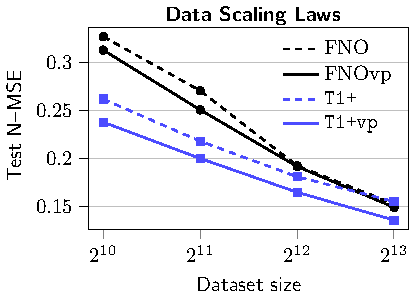
\includegraphics[width=\linewidth]{figures/scaling_law.pdf}
    \vspace{-5.5mm}
    \caption{\small Scaling laws for N-MSE.}
    \label{fig:scaling_law}
\end{wrapfigure}
%
We verify whether the reduction in predictive error of \ourmethod{} over neural operator baselines is preserved as the size of training dataset grows. We perform $10$ training runs on the Navier-Stokes $\nu=1e^{-4}$ experiment, each time with a larger dataset size, and report the scaling laws in \cref{fig:scaling_law}. With additional data, the gaps in test errors narrow slightly, with noticeable improvements obtained by applying the {\tt vp} scheme to both FNO and {\tt T1+}.



\subsection{Flow Around Airfoils}\label{subsec:dfp}
%
We investigate the performance of \ourmethod{} in predicting steady-state solutions of flow around airfoils. 

\paragraph{Setup}

We use data introduced in \citep{thuerey2020deep} in the form of $10000$ training pairs of initial conditions, specifying freestream velocities and the airfoil mask, with the target steady-state velocity and pressure fields. This task introduces additional complexity in the form of higher resolution input images ($128$) and a full $k$-space due to the discontinuity in the field produced by the mask. 

We compare a SOTA UNet architecture (DFPNet) introduced by \citep{thuerey2020deep} to FNOs and \ourmethod{} with {\tt vp} initialization schemes. We perform a search on the most representative hyperparameters (detailed in the Appendix). Averages for $5$ runs are reported in \cref{tab:dfp}.

\paragraph{Results}

\begin{wraptable}[9]{l}{0.43\linewidth}
    \vspace{-2mm}
    \centering
    \begin{tabular}{c|c|c}\toprule
        \textbf{Method} & N-MSE & Time (hrs) \\
        \midrule
        DFPNet & $0.023$ & $\textbf{1.3}$\\ 
        FNO & $\textbf{0.020}$ & $6.0$\\ 
        \rowcolor{blue!4}
        \ourmethod{+}vp & $0.024$ & $\textbf{1.3}$\\
    \end{tabular}
    \vspace{-0.2mm}
    \caption{\small Test N-MSE and total training time on the flow around airfoil task.}
    \label{tab:dfp}
\end{wraptable}

All models are able to accurately predict steady-state solutions for different airfoils with small normalized errors. Test N-MSE is comparable as all models are within a single standard deviation. Training of \ourmethod{} is as fast as DFPNets \citep{thuerey2020deep} and as accurate as FNOs, as evidence of the applicability of \ourmethod{} to tasks with signals that are not band-limited (in this case due to the airfoil mask).


\clearpage

\subsection{Turbulent Smoke}\label{subsec:scal}
We investigate the performance of \ourmethod{} in predicting iterative rollouts from high-resolution video of real rising smoke plumes.

\begin{minipage}[t]{\linewidth}
    \centering
    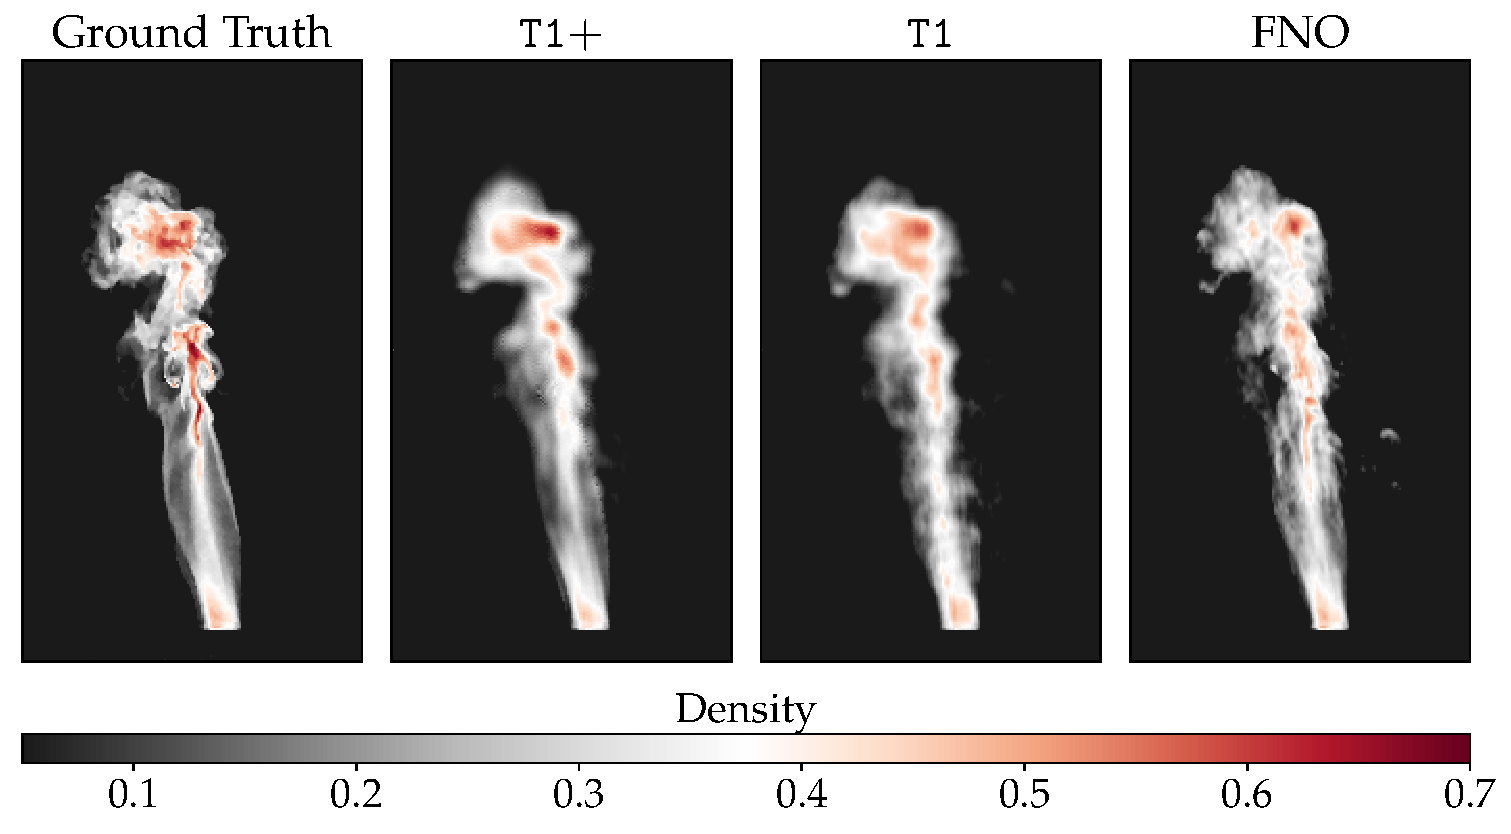
\includegraphics[width=0.49\linewidth]{figures/scalarflow_comparison_large.pdf}
    \hfill
    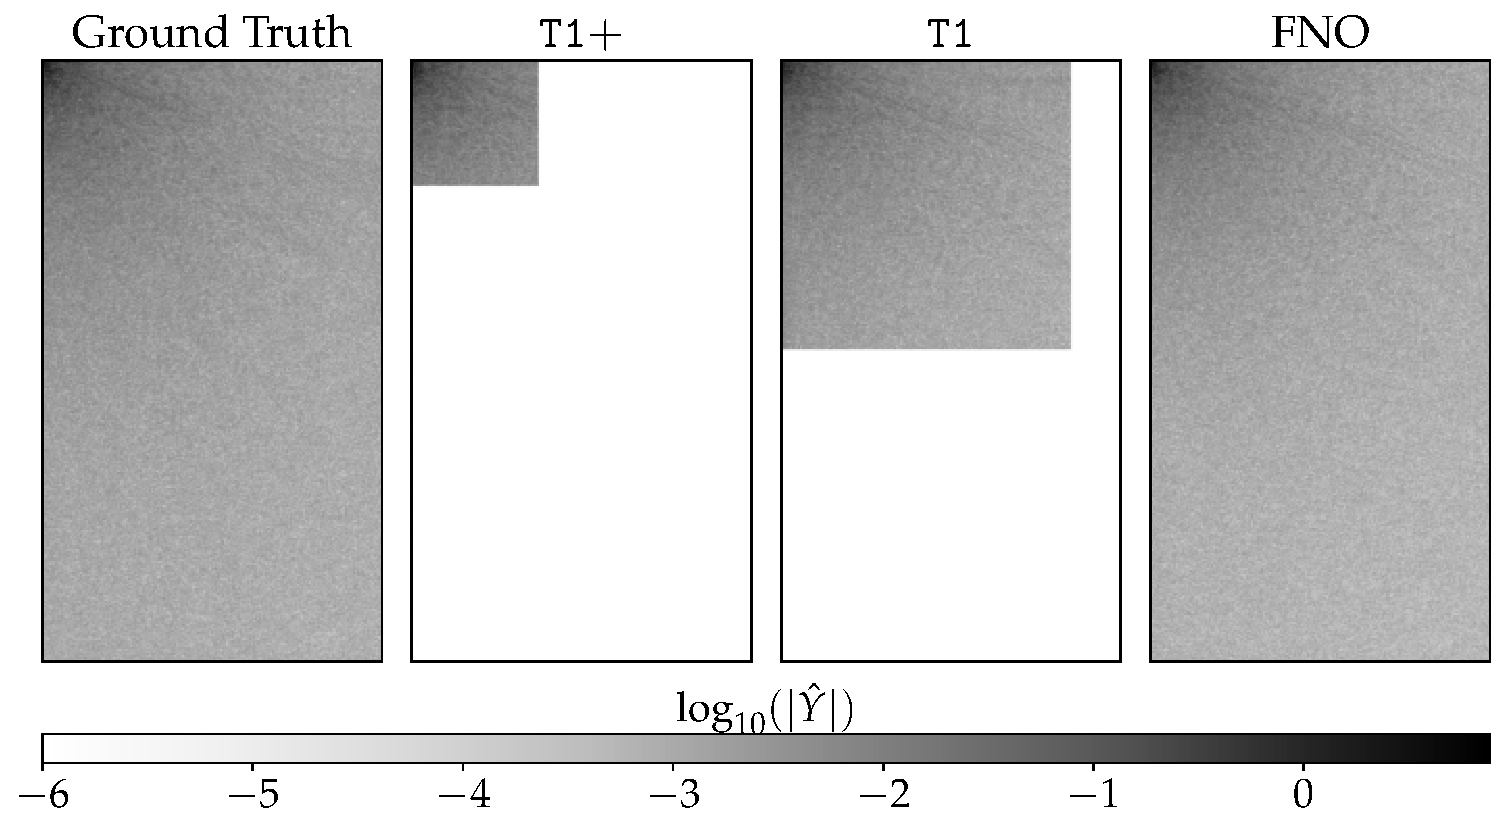
\includegraphics[width=0.49\linewidth]{figures/scalarflow_comparison_dct_large.pdf}
    \vspace{-3mm}
     \captionof{figure}{\small \textbf{[Left]} $10$-step rollout predictions on ScalarFlow. FNOs produce high-frequency, non-physical artifacts and accumulate error more rapidly in time compared to \ourmethod{} models \textbf{[Right]} Log-absolute values of predictions in $k$-space (DCT-II). Although \ourmethod{} is limited to $m=512$ and \ourmethod{+} to $m=224$ $k$-space elements, the predictions are overall more physically accurate in $n$-space.}
\label{fig:scalarflow-comparison-raw}
\end{minipage}
% \hfill

\paragraph{Setup}
We use the ScalarFlow dataset introduced in \citep{eckert2019scalarflow} consisting of $104$ sequences of $150$ frames each collected from video recordings of rising hot smoke plumes. The dataset consists of raw video data at high-resolution ($600$ × $1062$) collected at $60$ fps. This task scales up complexity by involving real-world high-definition data, capturing highly-turbulent dynamics. We perform rollouts iteratively based on previous predictions: all models are trained on $3$-step rollouts and evaluated over $10$-steps extrapolation to test their generalization in time. We compare FNOs against \ourmethod{}, \ourmethod{+} and \ourmethod{+vp} of similar model sizes after performing a search on most representative hyperparameters (Appendix B).

%  FNO models truncate to $m=48$ with residual connections, \ourmethod{} to $m=512$ and \ourmethod{+} to $m=224$.
 
 \begin{wraptable}[9]{r}{0.42\linewidth}
    \vspace{-3.6mm}
    \centering
    \begin{tabular}{c|c|c}\toprule
        \textbf{Method} & N-MSE & Time (hrs) \\
        \midrule
        FNO & $0.232$ & $32.4$\\ 
        \ourmethod{} & $0.239$ & $8.1$\\ 
        \ourmethod{+} & $0.256$ & $4.7$\\
        \rowcolor{blue!4}
        \ourmethod{+vp} & $\textbf{0.228}$ & $\textbf{4.7}$\\
    \end{tabular}
    \vspace{-1.1mm}
    \caption{\small Test 10-steps rollout $n$-space prediction errors (N-MSE)  and total training time on the ScalarFlow dataset.}
    \label{tab:scalarflow-small}
\end{wraptable}


\paragraph{Results}
\cref{fig:scalarflow-comparison-raw} provides a sample rollout of different model predictions in $k$-space (DCT-II). \ourmethod{+vp} accumulates smaller errors over the rollout and is less prone to generating non-physical artifacts by performing prediction only on a subset of the $k$-space (\cref{tab:scalarflow-small}). Notably, \ourmethod{} and \ourmethod{+} are $4\times$ to $7\times$ faster, providing a reduction in training time from $32.4$ hours to $4.7$. Appendix B includes additional visualizations, including averaged prediction errors on $k$-space. 


\section{Conclusion}

We present a streamlined class of \textit{frequency domain models} (FDM): \textit{Transform Once} (\ourmethod{}). \ourmethod{} models are optimized directly in frequency domain, after a single transform, and achieve similar or improved predictive performance at a fraction of the computational cost ($3$x to $10$x speedups across tasks). Further, a simple truncation-aware weight initialization scheme is introduced and shown to improve the performance of \ourmethod{} and existing FDMs.

\section*{Acknowledgments}
This work is supported by NSF (1651565), AFOSR (FA95501910024), ARO (W911NF-21-1-0125), ONR, DOE, CZ Biohub, Sloan Fellowship and JSPS Kakenhi (21J14546).